\chapter{Preliminary Evaluation}
\label{sec:evaluation}

I converted two existing C benchmark suites as an initial evaluation
of the consequences of porting code to Checked C (with assistance from
David Tarditi and researchers at Samsung Research). We quantify both
the changes required for the code to become checked, and the overhead
imposed on compilation, running time, and executable size.

\section{Benchmarks}

\begin{table}[ht]
% Table: A Description of our Benchmarks
\centering
\begin{tabular}{lrl}
\toprule
Name           & \multicolumn{1}{c}{LoC} & Description                                             \\
\midrule
bh             & 1,162 & Barnes \& Hut N-body force computation algorithm        \\
bisort         & 262   & Sorts using two disjoint bitonic sequences              \\
em3d           & 476   & Simulates electromagnetic waves in 3D                   \\
health         & 338   & Simulates Colombian health-care system                  \\
mst            & 325   & Computes minimum spanning tree using linked lists       \\
perimeter      & 399   & Computes perimeter of a set of quad-tree encoded images \\
power          & 452   & The Power System Optimization problem                   \\
treadd         & 180   & Computes the sum of values in a tree                    \\
tsp            & 415   & Estimates solution for the Traveling-salesman problem   \\
\emph{voronoi} & 814   & Computes voronoi diagram of a set of points             \\
\addlinespace
anagram        & 346   & Generates anagrams from a list of words                 \\
\emph{bc}      & 5,194 & An arbitrary precision calculator                       \\
ft             & 893   & Computes minimum spanning tree using Fibonacci heaps    \\
ks             & 549   & Schweikert-Kernighan graph partitioning                 \\
yacr2          & 2,529 & VLSI channel router                                     \\
\bottomrule
\end{tabular}
\caption{Compiler Benchmarks. Top group is the Olden suite, bottom
group is the Ptrdist suite. LoC includes all comments and blank lines
in benchmark source files. Descriptions are from
\cite{Rogers1995Olden,Austin1994Ptrdist}. We were unable to convert
\emph{voronoi} from the Olden suite and \emph{bc} from the Ptrdist suite using the current version of
Checked C.}
\label{tab:bmdesc}
%%% Local Variables:
%%% mode: latex
%%% TeX-master: "../tr02"
%%% End:

\end{table}

I chose the Olden \cite{Rogers1995Olden} and Ptrdist
\cite{Austin1994Ptrdist} benchmark suites, described in
Table~\ref{tab:bmdesc}, because they are specifically designed to test
pointer-intensive applications, and they are the same benchmarks used
to evaluate both Deputy~\cite{Feng2006} and CCured~\cite{Necula2005}.

We evaluate Checked C using these benchmarks in two ways. First, we
quantify the number and type of source code changes required to
convert these benchmarks from C to Checked C. Second, we quantify the
overhead of the run-time checks on benchmark run time, compile time,
and executable size. The evaluation results are presented in
Table~\ref{tab:bmresults}.

\paragraph{Experimental Setup} These were produced using a 12-Core
Intel Xeon X5650 2.66GHz, with 24GB of RAM, running Red Hat Enterprise
Linux 6. All compilation and benchmarking was done without
parallelism. We ran each benchmark 21 times with and without the
Checked C changes using the test sizes from the LLVM versions of these
benchmarks. We report the median; we observed little variance.

\paragraph{Excluded Benchmarks} We were unable to convert the
\emph{voronoi} benchmark from the Olden suite due to bounds
propagation limitations detailed in~\autoref{sec:prop-limitations}. We
were unable to convert the \emph{bc} from the Ptrdist suite due to
lack of time. They are excluded from any conversion results.

\begin{table}[ht]
% Table of benchmark results
\centering
\begin{tabular}{lrrrrrr}
\toprule
          & \multicolumn{3}{c}{Code Changes}
          & \multicolumn{3}{c}{Observed Overheads} \\
\addlinespace
Benchmark
          & \multicolumn{1}{c}{\emph{LM} \%}
          & \multicolumn{1}{c}{\emph{EM} \%}
          & \multicolumn{1}{c}{\emph{LU} \%}
          & \multicolumn{1}{c}{\emph{RT} $\pm$\%}
          & \multicolumn{1}{c}{\emph{CT} $\pm$\%}
          & \multicolumn{1}{c}{\emph{ES} $\pm$\%} \\
\midrule
bh & 10.0 & 76.7 & 5.2 & + 0.2 & + 23.8 & + 6.2 \\
bisort & 21.8 & 84.3 & 7.0 & 0.0 & + 7.3 & + 3.8 \\
em3d & 35.3 & 66.4 & 16.9 & + 0.8 & + 18.0 & - 0.4 \\
health & 24.0 & 97.8 & 9.3 & + 2.1 & + 18.5 & + 6.7 \\
mst & 30.1 & 75.0 & 19.3 & 0.0 & + 6.3 & - 5.0 \\
perimeter & 9.8 & 92.3 & 5.2 & 0.0 & + 4.9 & + 0.8 \\
power & 15.0 & 69.2 & 3.9 & 0.0 & + 21.6 & + 8.5 \\
treadd & 17.2 & 92.3 & 20.4 & + 8.3 & + 83.1 & + 7.0 \\
tsp & 9.9 & 94.5 & 10.3 & 0.0 & + 47.6 & + 4.6 \\
\addlinespace
anagram & 26.6 & 67.5 & 10.7 & + 23.5 & + 16.8 & + 5.1 \\
ft & 18.7 & 98.5 & 6.3 & + 25.9 & + 16.5 & + 11.3 \\
ks & 14.2 & 93.4 & 8.1 & + 12.8 & + 32.3 & + 26.7 \\
yacr2 & 14.5 & 51.5 & 16.2 & + 49.3 & + 38.4 & + 24.5 \\
\midrule
\multicolumn{1}{r}{Geo. Mean:} & 17.5 & 80.1 & 9.3 & + 8.6 & + 24.3 & + 7.4 \\

\bottomrule
\end{tabular}
\caption{Benchmark Results. Key: \emph{LM~\%}:
Percentage of Source LoC Modified, including Additions; \emph{EM~\%}:
Percentage of Code Modifications deemed to be Easy (see
\ref{sec:eval-code-changes}); \emph{LU~\%}: Percentage of Lines
remaining Unchecked; \emph{RT~$\pm$\%}: Percentage Change in Run Time;
\emph{CT~$\pm$\%}: Percentage Change in Compile Time;
\emph{ES~$\pm$\%}: Percentage Change in Executable Size
(\texttt{.text} section only)}
\label{tab:bmresults}


%%% Local Variables:
%%% mode: latex
%%% TeX-master: "../tr02"
%%% End:

\end{table}

\section{Code Modifications}
\label{sec:eval-code-changes}

\begin{figure}[ht]
\centering
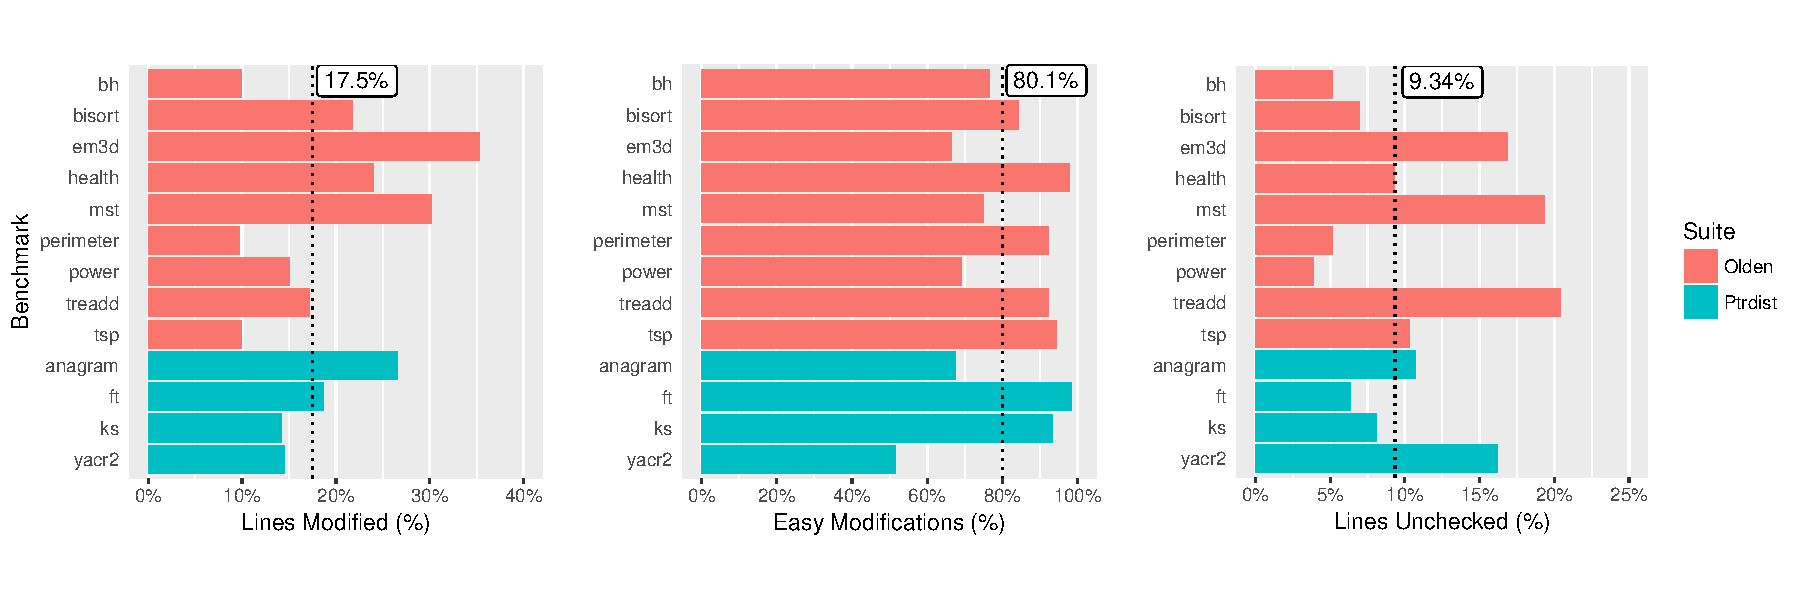
\includegraphics[width=\linewidth]{scripts/modifications}
\caption{Code Modifications}
\label{fig:cm-plot}
\end{figure}

On average, the changes modified \ResultLinesModifiedMean of benchmark
lines of code. Most of these changes were in declarations,
initializers, and type definitions rather than in the program logic.
In the evaluation of Deputy~\cite{Condit2007}, the reported figure of
lines changed ranges between 0.5\% and 11\% for the same benchmarks,
showing they have a lower annotation burden than Checked C.

We modified the benchmarks to use checked blocks and the top-level
checked pragma. We placed code that could not be checked because it
used unchecked pointers, or assignments where our static analysis
could not currently verify that the assignment was valid, in unchecked
blocks. On average, about \ResultLinesUncheckedMean of the code
remained unchecked after conversion, with a minimum and maximum of
\ResultLinesUncheckedMin and \ResultLinesUncheckedMax. The causes were
almost entirely variable argument functions such as
\lstinline|printf|.

We manually inspected changes and divided them into \emph{easy}
changes and \emph{hard} changes. Easy changes include:

\begin{itemize}
\item replacing included headers with their checked versions;
\item converting a \uncheckedptrT{} to a \PtrT{};
\item adding the \kwchecked{} keyword to an array declaration;
\item introducing a \kwchecked{} or \kwunchecked{} region;
\item adding an initializer; and
\item replacing a call to \lstinline|malloc| with a call to
\lstinline|calloc|.
\end{itemize}

Hard changes are all other changes, including changing a
\uncheckedptrT{} to a \ArrayptrT{} and adding a bounds declaration,
adding structs, struct members, and local variables to represent
run-time bounds information, and code modernization.

We distinguish between the two because we believe easy changes can be
automated (as with our automated \PtrT{} conversion tool) or made
unnecessary in the future by relaxing requirements such as the
additions of initializers.

In all of our benchmarks, we found the majority of changes were easy.
In six of the benchmarks, the only hard changes were adding bounds
annotations relating to the parameters of \lstinline|main|. In yacr2
there are a lot of bounds declarations that are all exactly the same
where global variables are passed as arguments, inflating the number
of ``hard'' changes.

\paragraph{Layout Changes} In three benchmarks---em3d, mst, and
yacr2---we had to add intermediate structs so that we could represent
the bounds on \ArrayptrT{}s nested inside arrays. In mst we also had
to add a member to a struct to represent the bounds on an
\ArrayptrT{}. In the first case, this is because we cannot represent
the bounds on nested \ArrayptrT{}s, in the second case this is because
we only allow bounds on members to reference other members in the same
struct. In em3d and anagram we also added local temporary variables to
represent bounds information.

\section{Performance Results}

\begin{figure}[ht]
\centering
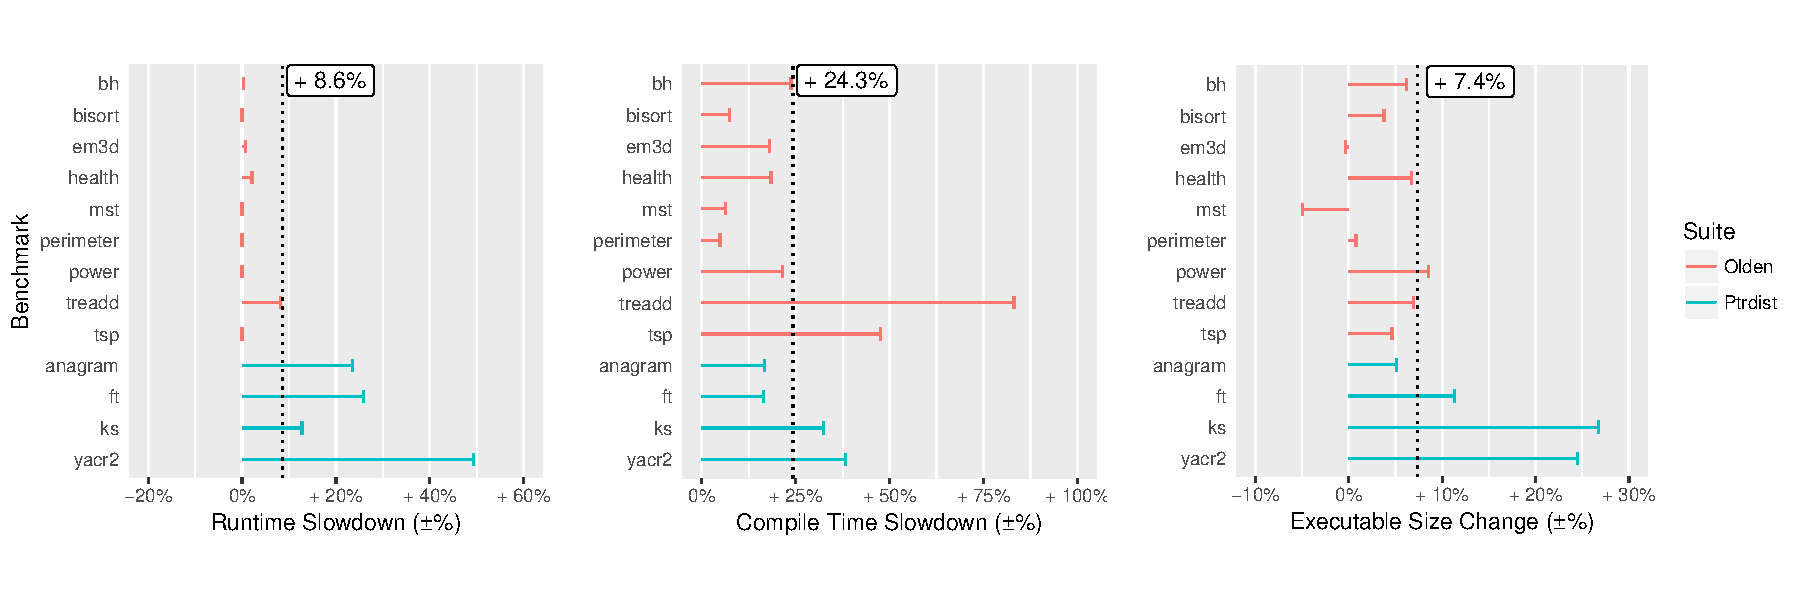
\includegraphics[width=\linewidth]{scripts/overheads}
\caption{Performance Overheads}
\label{fig:oh-plot}
\end{figure}

An important concern about run-time checking for C is the effect on
performance and compile time. The average run-time overhead introduced
by added dynamic checks was \ResultRunTimeMean. In more than half of
the benchmarks the overhead was less than 1\%. We believe this to be
an acceptably low overhead that better static analysis may reduce even
further.

In all but two benchmarks---treadd and ft---the added overhead matches
(meaning performance is within 2\% of) or betters that of Deputy. For
yacr2 and em3d, Checked C does substantially better than Deputy, whose
overheads are 98\% and 56\%, respectively. Checked C's overhead
betters or matches that reported by CCured in every case but ft.

On average, the compile-time overhead added by using Checked C is
\ResultCompileTimeMean. The maximum overhead is \ResultCompileTimeMax,
and the minimum is \ResultCompileTimeMin faster than compiling with C.
We have spent no time at all optimising compile-time for Checked C. In
particular, treeadd is a major outlier because the program is so
short.

We also evaluated code size overhead, by looking at the change in the
size of \lstinline|.text| section of the executable. This excludes data
that might be stripped, like debugging information. Across the
benchmarks, there is an average \ResultExecutableSizeMean code size
overhead from the introduction of dynamic checks. Ten of the programs
have a code size increase of less than 10\%.

\section{Evaluation}

All considered, we offer equivalent or better performance than either
CCured or Deputy provide, at the outlay of having to convert a larger
amount of code. We believe this to be a good trade-off, partially
because we feel most of these changes can be automated, and partially
because we provide the programmer greater control over how they
express their bounds in terms of other program data. The latter in
particular allows the programmer to work with their optimizer to
ensure run-time overhead, especially in tight loops, remains low.

\subsection{Interaction with the LLVM Optimizer}

Currently we have done no specific work within our compiler to elide
or optimize our dynamic checks. Any checks that Clang/LLVM currently
removes, it does so using its existing optimization passes.

We expected the LLVM optimizer to be a lot worse at optimizing dynamic
checks than it turned out to be. In only two of our benchmarks did we
have to hand-optimize these programs to reduce the overhead of dynamic
checking to approximately 0\%. This was accomplished by a mixture of
being more specific with annotated bounds (including introducing
temporary variables) and hoisting checks from inner loops using
explicit dynamic checks.

Expressions that caused most difficulty for removing dynamic checks
was code involving (at least) two pointer dereferences, as this incurs
an unavoidable non-null check on the inner pointer, even if the outer
pointer can be proven to be non-null. This can cause overhead in loops
iterating through, for example, linked lists or graphs. We are working
on a proposal to add nullness (and non-null) annotations to pointers
in Checked C, which would allow for these inner non-null checks to be
elided in many cases.

%%% Local Variables:
%%% mode: latex
%%% TeX-master: "tr02"
%%% End:
